
\documentclass[journal]{IEEEtran}

\IEEEoverridecommandlockouts                              % This command thanks command
%\overrideIEEEmargins
% See the \addtolength command later in the file to balance the column lengths
% on the last page of the document

%\def\baselinestretch{0.9999}

%\input{boldfacemath}

%\usepackage{exsheets}



% save and then undefine the offending command
% we need \makeatletter because \@undefined uses the special @ character.
\makeatletter
\let\IEEEproof\proof
\let\IEEEendproof\endproof
\let\proof\@undefined
\let\endproof\@undefined
\makeatother

% The following packages can be found on http:\\www.ctan.org
%\usepackage{graphics} % for pdf, bitmapped graphics files
%\usepackage{epsfig} % for xpostscript graphics files
%\usepackage{mathptmx} % assumes new font selection scheme installed
%\usepackage{times} % assumes new font selection scheme installed
\usepackage{amsmath} % assumes amsmath package installed
\usepackage{amssymb}  % assumes amsmath package installed
\usepackage{amsthm}
\usepackage{amsfonts}
\usepackage{mathtools}

% Text
\usepackage{comment}
\usepackage[normalem]{ulem}
%\usepackage[inline]{enumitem}
%let\labelindent\relax % Since the \labelindent command exists for legacy reasons in the IEEE template, you can simply "disable" it by adding the following before importing the enumitem package
%\usepackage{enumitem}
\usepackage{bm}
\providecommand{\bm}{\pmb}

%\usepackage{flushend}

\newtheorem{prop}{Proposition}
\newtheorem{cor}{Corollary}
\newtheorem{defin}{Definition}
\newtheorem{fact}{Fact}
\newtheorem{thm}{Theorem}[section]
\newtheorem{lem}[thm]{Lemma}
\newtheorem*{Zorn}{Zorn’s Lemma}
\theoremstyle{definition}
\newtheorem{dfn}{Definition}
\theoremstyle{remark}
\newtheorem*{rmk}{Remark}
\newtheorem{theorem}{Theorem}[section]
\newtheorem{remark}[theorem]{Remark}

\newtheorem{problem}{Problem}

\usepackage{verbatim}

\usepackage{color}
%\usepackage{subfig}
\usepackage{graphicx}
%\usepackage{caption}
\usepackage{esvect}



%\usepackage{mathptmx}
\usepackage{times}

%%%%%%%%%%%%%%%%%%%%%%%%%%%%%%%%%%%%%%%%%%%%%

\usepackage[ruled,vlined,linesnumbered]{algorithm2e}
%\usepackage[noend]{algorithmic}
\usepackage{algorithmicx}
\usepackage{algpseudocode}

%%%%%%%%%%%%%%%%%%%%%%%%%%%%%%%%%%%%%%%%%%%%%
\graphicspath{{images/}}

\usepackage[us]{datetime}
\usepackage{caption}
\captionsetup{font=small}


%\documentclass[a4, 10pt, conference]{ieeeconf}

 \usepackage[usenames,dvipsnames,table]{xcolor}

\usepackage{hyperref} %pdf with links and toc on the left
\hypersetup{
    colorlinks,
    citecolor=black,
    filecolor=black,
    linkcolor=black,
    urlcolor=black,
    pdfauthor={},
    pdfsubject={},
    pdftitle={}
}

\usepackage{todonotes}
%\usepackage{todonotes} lets you insert notes of stuff to do with the syntax \todo{Add details.}

\usepackage{graphicx}
% \usepackage{graphicx} manage external pictures

\usepackage{latexsym}
\usepackage{color}
% \usepackage{color} adds support for colored text

\usepackage{cite}

% \usepackage{cite} assists in citation management

\usepackage{caption}
%\usepackage{caption} allows customization of appearance and placement of captions for figures, tables, etc.
%\usepackage{subcaption}
\usepackage{subfig}


\usepackage{tikz}
\usepackage{adjustbox}
\usetikzlibrary{shapes,arrows}

% ---------- added packages -----------------------------------
\usepackage{tabularx, booktabs}
\newcolumntype{Y}{>{\centering\arraybackslash}X}
\usepackage{multirow}
\usepackage{paralist}
% ---------- New Symbols and Commands -------------------------
\usepackage{accents}
% ---------- Standard Commands ------------------

\usepackage{color}
\newcommand\red[1]{{\textcolor{red}{#1}}}
\newcommand\blue[1]{{\textcolor{blue}{#1}}}

\newcommand{\DS}[1]{\red{DS: #1}}
\newcommand{\MANU}[1]{\blue{MANU: #1}}
% ---------- new variables ------------------
\newcommand{\Hinf}{$H_\infty$\xspace}
\newcommand{\photoa}{PH-A}
\newcommand{\photob}{PH-B}
\newcommand{\photodistance}{d}


% ---------- new commands ------------------
\newcommand{\vect}[1]{\bm{#1}}		% vectors
\newcommand{\matr}[1]{\bm{#1}}		% matrices
\newcommand{\nR}[1]{\mathbb{R}^{#1}}		% real number
\newcommand{\nT}[1]{\mathbb{T}^{#1}}		% real number
\newcommand{\define}{:=}			% define symbol
\newcommand{\modulus}[1]{\left| #1 \right|}	% abs
\newcommand{\matrice}[1]{\begin{bmatrix} #1 \end{bmatrix}}	% matrix
\newcommand{\smallmatrice}[1]{\left[\begin{smallmatrix} #1 \end{smallmatrix}\right]}	% matrix
\newcommand{\cosp}[1]{\cos \left( #1 \right)}	% cos with brace
\newcommand{\sinp}[1]{\sin \left( #1 \right)}	% sin with brace
\newcommand{\determinant}[1]{\text{det}\left(#1\right)} 	% determinant
\newcommand{\sgn}[1]{\text{sgn}\left( #1 \right)}			% signum
\newcommand{\atanTwo}[1]{{\rm atan2}\left( #1\right)}		% atan2
\newcommand{\acotTwo}[1]{{\rm acot2}\left( #1\right)}		% acot2
\newcommand{\upperRomannumeral}[1]{\uppercase\expandafter{\romannumeral#1}}	% roman numbers
\newcommand{\lowerromannumeral}[1]{\romannumeral#1\relax}
\newcommand{\vSpace}{\;\,}
\newcommand{\ubar}[1]{\underaccent{\bar}{#1}}

%-----------Functions------------------------
\newcommand{\minEig}[1]{\lambda_{\text{min}}[#1]}
\newcommand{\maxEig}[1]{\lambda_{\text{max}}[#1]}
\newcommand{\transp}{^\top}


% --------- References ----------------------
\newcommand{\fig}{Fig.~}	% figure ref
\newcommand{\eqn}{Eq.~}	% equation ref
\newcommand{\tab}{Tab.~}	% table ref
\newcommand{\cha}{Chap.~}	% chapter ref
\newcommand{\sect}{Sec.~}	% section ref
\newcommand{\alg}{Algorithm~}

% --------- Variables -----------------------

% General
\renewcommand{\frame}{\mathcal{F}}		% frame
\newcommand{\origin}{O}						% origin
\newcommand{\vX}{\vect{x}}					% x-axis
\newcommand{\vY}{\vect{y}}					% y-axis
\newcommand{\vZ}{\vect{z}}					% z-axis
\newcommand{\pos}{\vect{p}}				% position vector
\newcommand{\dpos}{\vect{v}}				% velocity vector
\newcommand{\rotMat}{\matr{R}}				% rotation matrix
\newcommand{\rotMatVectAngle}[2]{\rotMat_{#1}(#2)}	% rotation matrix representing the rotation about a vector of a certain angle
\newcommand{\vZero}{\vect{0}}				% vect/matr of zeros
\newcommand{\en}[1]{\vect{e}_{#1}}		% vect e_n
\newcommand{\eye}[1]{\matr{I}_{#1}}
\newcommand{\zeros}[1]{\matr{0}_{#1}}
\newcommand{\skewmatr}[1]{\big[{#1}\big]_\times}
\newcommand{\skewmatrS}[1]{\matr{S}({#1})}

% World frame
\newcommand{\frameW}{\frame_W}			% world frame
\newcommand{\originW}{\origin_W}		% origin world frame
\newcommand{\xW}{\vX_W}				% x-axis world frame
\newcommand{\yW}{\vY_W}				% y-axis world frame
\newcommand{\zW}{\vZ_W}				% z-axis world frame
\newcommand{\dxW}{\dot{\vX}_W}

% Background
\newcommand{\samplingPeriod}{T_s}
\newcommand{\samplingFrequency}{f_s}
\newcommand{\vwater}{\bar{v}_{water}}
\newcommand{\vhex}{\bar{v}_{hex}}
\newcommand{\vfluid}{\bar{v}_{fl}}
\newcommand{\samplesWater}{N_{water}}
\newcommand{\samplesHex}{N_{hex}}
\newcommand{\samplesfl}{N_{fl}}
\newcommand{\samplesflk}{N_{fl,k}}
\newcommand{\samples}{n}
\newcommand{\avgL}[1]{L_{#1}}
\newcommand{\vnominal}{v_{n}}
\newcommand{\channelArea}{A}
\newcommand{\slugvelocity}{v_{sl}}


% Modeling 2nd Order Systems
\newcommand{\settlingtime}{t_s}
\newcommand{\naturalfrequency}{w_n}
\newcommand{\damping}{\xi}
\newcommand{\bias}{b_{0}}

% Modeling
\newcommand{\eigenvalues}[1]{\lambda_{#1}}
\newcommand{\slugfrequencyerror}{e_{\slugfrequency}}

% Flow rates
\newcommand{\flowratecommand}{F^{\star}_{fl}}
\newcommand{\flowrate}{F}
\newcommand{\flowratewatercommand}{F^{\star}_{water}}
\newcommand{\flowratehexcommand}{F^{\star}_{hex}}
\newcommand{\urate}{u_{fl}}
\newcommand{\uratess}{\expectedflowrate}
\newcommand{\urateinit}{u_{fl_{0}}}

\newcommand{\uratecommand}{\urate^{\star}}
\newcommand{\uratecommandwater}{u^{\star}_{water}}
\newcommand{\uratecommandhex}{u^{\star}_{hex}}
\newcommand{\out}{y}


% Frequency
\newcommand{\slugfrequency}{f_{sl}}
\newcommand{\slugfrequencyinit}{f_{sl_{0}}}
\newcommand{\slugfrequencyss}{\tilde{f}_{sl}} %steady-state
\newcommand{\currentslugfrequency}{f_{sl}^c}
\newcommand{\desiredslugfrequency}{f_{sl}^d}
\newcommand{\slugfrequencyDes}{\desiredslugfrequency} %easy to use command wrt desiredsslugfrequency. This is the reason of the repetition.

% Control
\newcommand{\samplesk}{k}
\newcommand{\modelgain}{K_p}
\newcommand{\predictionHorizon}{N_p}
\newcommand{\controlHorizon}{N_c}
\newcommand{\controlVector}{\Delta \matr{U}}
\newcommand{\controlvector}[1]{\Delta \uratecommand({#1})}
\newcommand{\controlsample}{\uratecommand}
\newcommand{\referenceVector}{\matr{R}_{\slugfrequency}}
\newcommand{\outputVector}{\matr{Y}}
\newcommand{\outputvector}[1]{y_{fl}(#1)}
\newcommand{\costfunction}{\matr{J}}
\newcommand{\performanceMatrix}{\bar{\matr{R}}}
\newcommand{\slugfrequencymean}{\mu_{\slugfrequency}}
\newcommand{\slugfrequencystd}{\sigma_{\slugfrequency}}
\newcommand{\expectedflowrate}{\tilde{u}_{fl}}

\newcommand{\transitionMatrix}{\matr{F}}
\newcommand{\controlMatrix}{\matr{\Phi}}
\newcommand{\state}{x} 
\newcommand{\timeWindow}{t_w}


%My symbols
\newcommand{\abscissa}{x}
\newcommand{\ordinate}{y}
\newcommand{\mean}[1]{<V_{#1}(t)>}
\newcommand{\meann}{<V(t)>}
\newcommand{\spatialmean}[3]{V_{#1}({#2},{#3},t)}
\newcommand{\width}{W_{ROI}}
\newcommand{\height}{H_{ROI}}
\newcommand{\frequency}{f_i}
\newcommand{\amplitude}{A}
\newcommand{\range}{Range<V_x(t)>}
\newcommand{\peak}{AP}
\newcommand{\particles}{<N_p(t)>}

%Measurement units
\newcommand{\pixel}{pixels}
\newcommand{\apixel}{pixel}
\newcommand{\density}{Kg/m^3}
\newcommand{\hertz}{Hz}
\newcommand{\flow}{ml/min}
\newcommand{\seconds}{s}
\newcommand{\framerate}{FPS}
\DeclarePairedDelimiter{\norm}{\lVert}{\rVert} % norm

\captionsetup[subfigure]{labelformat=simple, labelsep=colon}
\makeatletter
\renewcommand*{\thesubfigure}{(\alph{subfigure})} 
\makeatother
%\makeatother
\pagestyle{headings}

%%%%%%%%%%%%%%%%%%%%%%%%%%%%%%%%%%%%%%%%%%%%%%%%%%%%%%%%%%%%%%%%%%%%%%%%%%%%%%%

\title{DPIV Analysis and Real Time Implementation}


\author{E. Cutuli${^{1}}$, G. Stella${^{1}}$, D. Sanalitro${^{1}}$, M. Bucolo${^{1}}$~\IEEEmembership{Senior Member,~IEEE}

\thanks{$^1$Department of Electrical Electronic and Computer Science Engineering, University of Catania, CT, Italy. {\tt \scriptsize\href{mailto:uni391076@studium.unict.it}{\mbox{uni391076@studium.unict.it}}
\scriptsize\href{mailto:emaunuela.cutuli@phd.unict.it}{\mbox{emanuela.cutuli@phd.unict.it}}
\scriptsize\href{mailto:giovanna.stella@phd.unict.it}{\mbox{giovanna.stella@phd.unict.it}}
\scriptsize\href{mailto:dario.sanalitro@unict.it}{\mbox{dario.sanalitro@unict.it}}}. 
\scriptsize\href{mailto:maide.bucolo@unict.it}{\mbox{maide.bucolo@unict.it}}}. 
}

%\thanks{Digital Object Idenitifier (DOI): see top of this page}




%%%%%%%%%%%%%%%%%%%%%%%%%%%%%%%%%%%%%%%%%%%%%%%%%%%%%%%%%%%%%%%%%%%%%%
\begin{document}
%%%%%%%%%%%%%%%%%%%%%%%%%%%%%%%%%%%%%%%%%%%%%%%%%%%%%%%%%%%%%%%%%%%%%%


\maketitle

%%%%%%%%%%%%%%%%%%%%%%%%%%%%%%%%%%%%%%%%%%%%%%%%%%%%%%%%%%%%%%%%%%%%%%
\begin{abstract}

\end{abstract}
%%%%%%%%%%%%%%%%%%%%%%%%%%%%%%%%%%%%%%%%%%%%%%%%%%%%%%%%%%%%%%%%%%%%%%

\begin{IEEEkeywords}
	Signal processing, Micro-optofluidic device, Data-driven Modelling
\end{IEEEkeywords}

\section{Introduction}

This paper ecc...



\section{Materials and Methods}

\subsection{System Design and Hardware Platform Realization}\label{sec:design}

From a methodological point of view, the experimental characterization of the process takes place through the acquisition of video signals that allow studying different interaction mechanisms between particles/cells subject to external hydrodynamic actuation.
The captured videos is then analyzed using the Digital Particle Image Velocimetry (DPIV).
\\From a hardware realization point of view, the focus is put on interfacing the microfluidic device with a video signal acquisition system.
Then different sources of actuation, mechanical by syringe pumps and optical by LED light are considered through which it is possible to study different interaction mechanisms between micro-particles subjected to different external stresses, in particular to sinusoidal flows with frequency and amplitude values to be fixed. 

\begin{figure}[h]
	\centering
	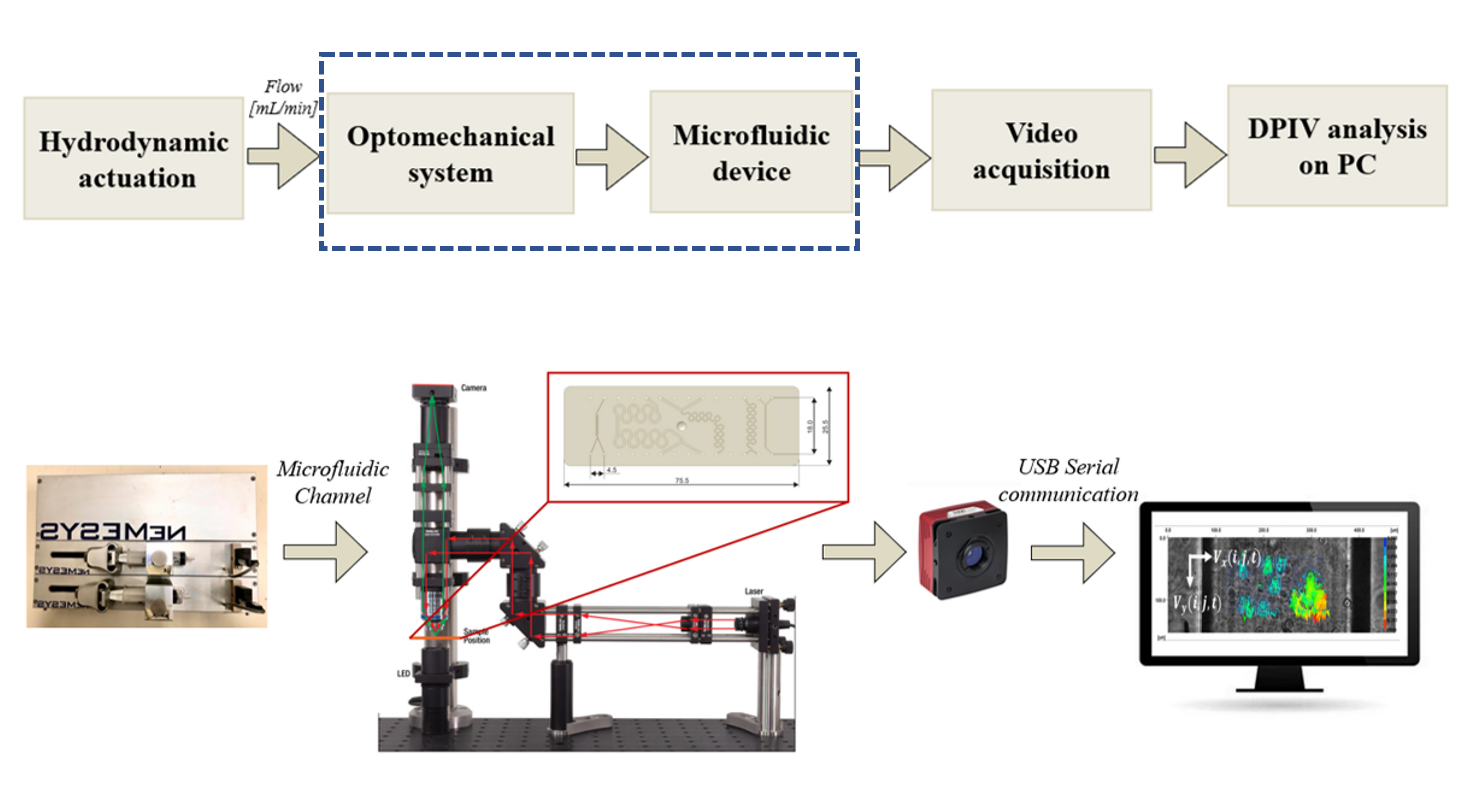
\includegraphics[width=1\columnwidth]{images/Platform}
	\centering{\caption{\label{Platoform}System Design and Hardware Platform Realization block schemes }}
\end{figure}

%$\flowrate$, $\flowratewatercommand$,$\channelArea$ are all examples of variables defined in "symbol-definition.tex"

\subsection{DPIV Online Platform Implementation}\label{sec:method}
In this paper, a DPIV online platform implementation for data acquisition and processing is proposed. Starting from a pre-existing DPIV platform that works offline, a new version of the same algorithm
that works online has been implemented. ~\fig\ref{Algorithms} shows a schematic of the two implementations. The feature that most diversifies the two algorithms is based on the fact that the offline algorithm works on a video acquired in a moment before the analysis that is carried out.

\begin{figure}[h]
	\centering
	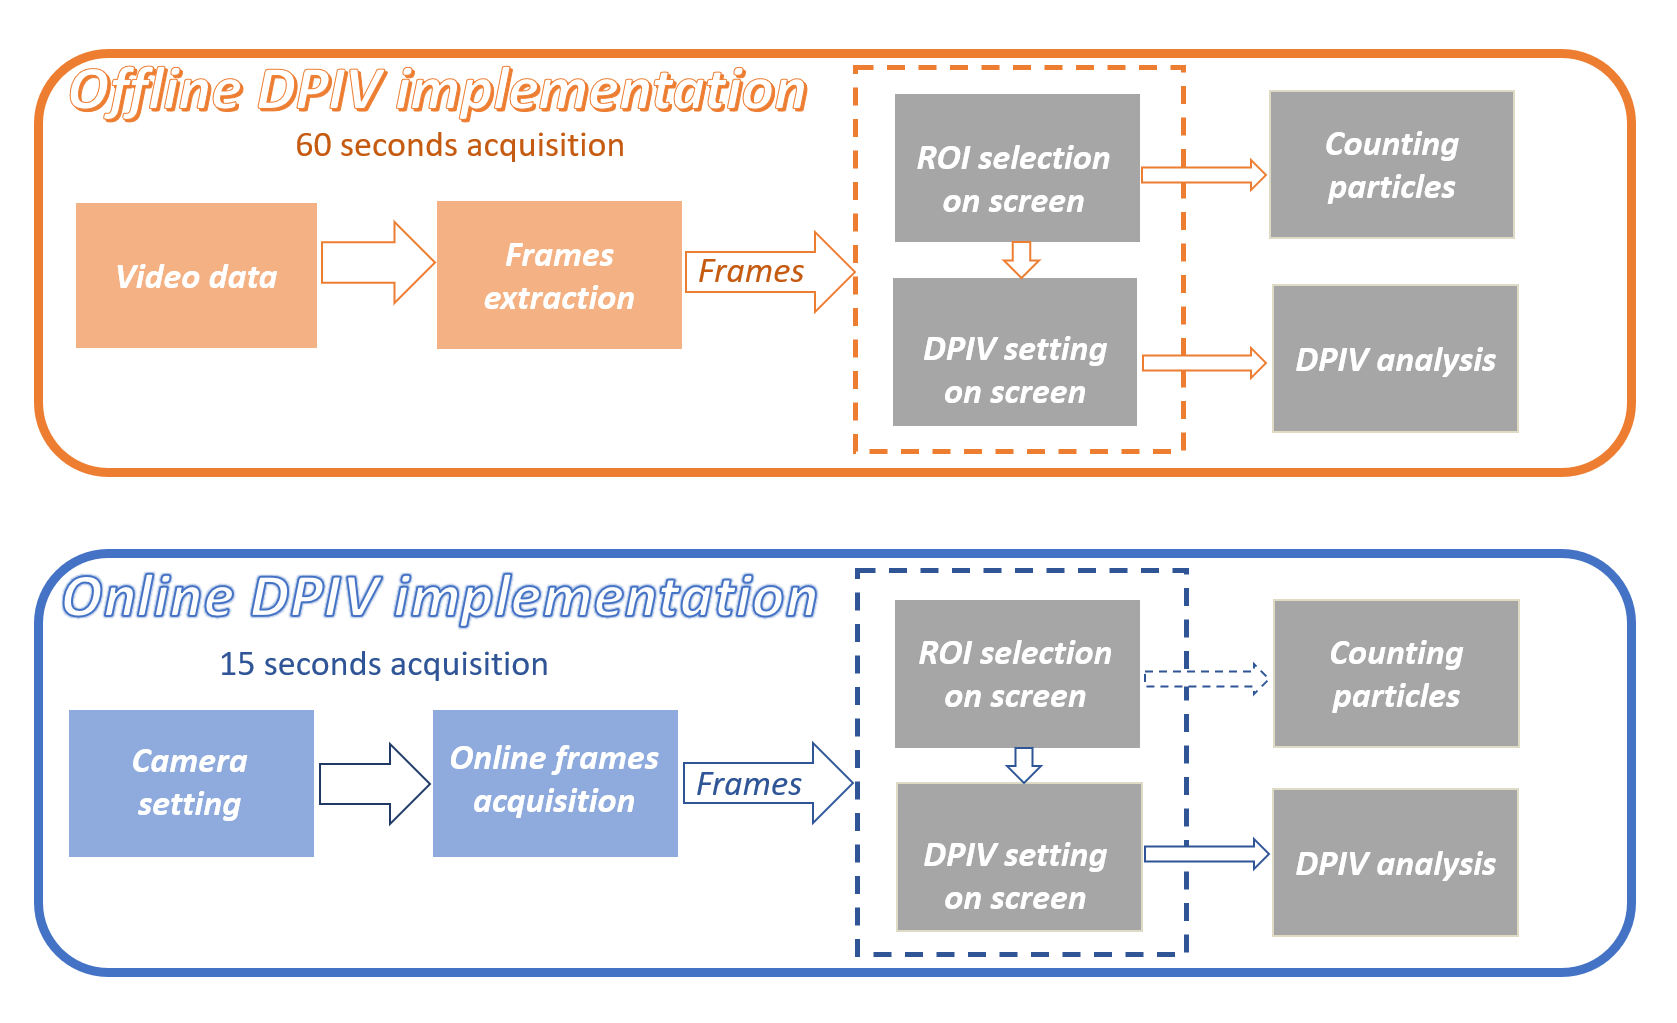
\includegraphics[width=1\columnwidth]{images/DPIV}
	\centering{\caption{\label{Algorithms}Offline and Online algorithms }}
\end{figure}

The first step involves the camera parameters setting, through the following quantities:

\begin{itemize}
	\item \textbf{Pixelsize}: obtained from the camera datasheet.
	\item \textbf{Magnification}: based on the optical components used in the experimental setup.
	\item \textbf{Exposure time}: chosen on the basis of experimental needs.
	\item \textbf{Image gain}: chosen on the basis of experimental needs.
\end{itemize}

Some simulations have been carried out to evaluate camera performances varying the parameters and the results found are listed below:
\begin{itemize}
	\item Increasing the Gain, the acquired image became clearer (see ~\fig\ref{CamPar}) without affecting the framerate.
	\item Increasing the Exposure time the acquired image became clearer (see ~\fig\ref{CamPar}) but this reduces a lot the framerate. 
	\\A compromise between the clarity of the image obtained by increasing the Exposure time and the framerate must be reached.
	\item If the Exposure Time is too small, even increasing the Gain, the image quality is bad.
\end{itemize}

\begin{figure}[h]
	\centering
	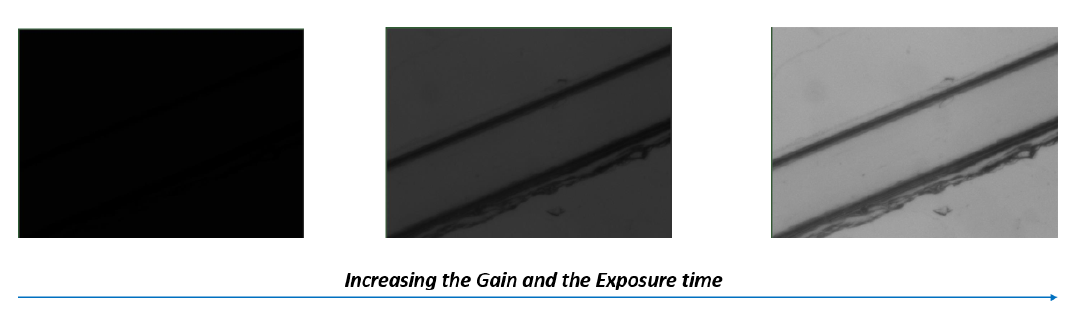
\includegraphics[width=1\columnwidth]{images/CameraParameters}
	\centering{\caption{\label{CamPar}Increase in image quality by acting on camera parameters }}
\end{figure}

The major contribution of this algorithm is represented by the acquisition that takes place in an online mode through the communication between the CCD camera and MATLAB downloading the \textbf{Windows SDK and Doc. for Scientific Cameras}.
\\Having the data available, the algorithm proceeds in a similar way to the offline case. The analyzes are carried out cyclically on sub-groups of frames, iteratively updating the results.
\\An on-screen ROI selection procedure has been introduced. It is determined by setting the left-top
corner of the image as the starting pixel and the right-down corner of the image as the end pixel, in order to obtain the desired width (W) and height (H). 
\\A DPIV analysis followed by a micro-particles counting procedure are at this point carried out for the predefined interrogation regions of interest (ROI). The DPIV approach consists of a first collection of the
time-varying velocity vector maps and a subsequent evaluation of the cross-correlation between ROIs of consecutive pairs of images. The velocity spatial distribution along the horizontal $V_x(i,j,t)$ and vertical $V_y(i,j,t)$ directions is obtained for each frame. Spatial averaging is done so that a single velocity value is obtained for each frame. By repeating this procedure for all the frames, two signals representing the trends of the average speed over time are given, respectively $<V_x(t)>$ and $<V_y(t)>$.
The preliminary step of DPIV setting concerns the possibility of opting to a multi-pass DFT for the DPIV analysis, through the following parameters: 

\begin{itemize}
	\item \textbf{Number of passes}: choosing form 1 to 4
	\item \textbf{Step Size}
	\item \textbf{Interrogation areas}: varying with to the first parameter
\end{itemize}

A multi-pass DFT could be used in order to increase the accuracy. A good compromise between the resolution and the computational time is given by the DFT approach with interrogation areas 64-32-16, so number of passes equal to 3, and step size 8. 
\\There is a further choice of performing the analysis in the whole ROI (single section) or by dividing the ROI into three horizontal sections, parallel to the particles' motion direction (three sections). This choice allows to highlight through the results the different particles average speed in the edges of the channel, which is greater than the one at the center of the channel.
\\The second type of analysis that this platform provides is the micro-particles counting.This procedure is based on highlighting the particles in the image distinguishing them from the background.
 \\The steps for the counting operation are:
 
 \begin{enumerate}
 	\item ROI selection;
 	\item Conversion to greyscale;
 	\item Duplication of the image;
 	\item Application of a gaussian filter (radius equal to 5);
 	\item Difference between the original image and the duplicated one;
 	\item Binarization of the image;
 \end{enumerate}
At this point a function takes as input the binary image. It traces the exterior boundaries of particles and gives the number of them found.
Important parameters to be set are the minimum and maximum dimensions of the cells, in order to count among the found objects only those that have an appropriate size, and a threshold value, chosen to define the circularity (a threshold equal to 1 indicates a perfect circle).



\section{Experiments}

\subsection{Experimental Setup}

\subsection{Experimental Results}

\subsubsection{Offline vs Online}

\subsubsection{Micro-Particles counting and velocity}

\paragraph{Particles suspended in fluids with different densities}

\paragraph{Viable cells, Dead cells and Synthetic Particles in comparison}

\section{Conclusions}


%\bibliographystyle{IEEEtran}
% DO NOT ERASE THE NEXT LINE,
% ONLY COMMENT IT AND DECOMMENT THE NEXT-NEXT, IF YOU NEED
%\bibliography{./bibCustom}



\end{document}

